% !TEX root = handbook-physics.tex
% !TEX TS-program = pdflatex
% !TEX encoding = UTF-8 Unicode






\chapter{Damped And Forced Oscillations}
\label{ch-29}
\zhtitle{阻尼振动与受迫振动}

\section{Damped Oscillations}
\label{sec-29.1} 
\zhtitle{阻尼振动}

\subsection{}\label{29.1.1} The \redem{damping of an oscillation or vibration} is its gradual weakening in the course of time due to the loss of energy of the oscillatory (vibratory) system. Free oscillations (vibrations) of real systems are always damped. The damping of free mechanical vibrations is due chiefly to friction and the excitation of elastic waves \ssect{30.1.3} in the surrounding medium. Damping in electrical oscillatory systems is due to thermal losses in the conductors making up the system or located in its variable electric field, energy losses on the radiation of electromagnetic waves \ssect{31.1.1}, and heat losses in dielectrics and ferromagnetic materials as a result of electrical and magnetic hysteresis \ssect{18.4.5} and \ssect{26.5.2}.
\zhpar{\redem{振动的阻尼}是指振动系统由于能量损失而使振动随时间逐渐减弱的现象。实际系统的自由振动总是有阻尼的。机械自由振动的阻尼主要源于摩擦以及周围介质中弹性波的激发（\ssect{30.1.3}）。电振荡系统中的阻尼则源于：组成系统的导体中以及处于其变化电场中的导体中的热损耗；电磁波辐射造成的能量损失（\ssect{31.1.1}）；以及电介质和铁磁材料中因电滞和磁滞而产生的热损耗（\ssect{18.4.5}和\ssect{26.5.2}）。}

The damping of oscillations depends upon the properties of the oscillatory system. A system is said to be \redem{linear} if the para­ meters characterizing physical properties of the system, essential in the process being considered, do not change in the course of the process. Linear systems are described by linear differential equations. A spring pendulum \ssect{28.2.3}, for instance, moving in a viscous medium, is a linear system if the resistance coefficient of the medium and the elasticity of the spring are independent of the velocity and displacement of the pendulum. An electrical oscillatory circuit \ssect{28.3.1} can be considered linear if its electrical resistance $R$, capacitance $C$ and inductance $L$ are independent of the current in the circuit, and the voltage. In the majority of cases real oscillatory or vibratory systems arc sufficiently close, with respect to their properties, to linear ones.
\zhpar{振动的阻尼取决于振动系统的性质。若描述系统物理性质的参量在所考虑的过程中保持不变，且这些参量对该过程起主要作用，则称该系统为\redem{线性}系统。线性系统用线性微分方程描述。例如，弹簧振子在粘性介质中运动时，若介质的阻力系数和弹簧的弹性都与振子的速度和位移无关，则它是线性系统。电振荡回路（\ssect{28.3.1}）若其电阻 $R$、电容 $C$ 和电感 $L$ 都与回路中的电流和电压无关，则可以视为线性系统。在大多数情况下，实际的振动或振荡系统在性质上与线性系统已足够接近。}

\subsection{}\label{29.1.2} \redem{The differential equation for the free damped oscillation of a linear system} is of the form:
\zhpar{\redem{线性系统自由阻尼振动的微分方程}具有如下形式：}
\begin{equation}%
\dv[2]{s}{t} + 2 \beta \dv{s}{t} + \omega_{0}^{2}s = 0.
\end{equation}
Here $s$ is the physical characteristic of the system that varies in the oscillation, $\beta = \text{const.} > 0$ is the \redem{damping factor}, and $\omega_{0}$ is the angular frequency of free \redem{undamped} oscillation of the same system, i.e. in the absence of energy losses (at $\beta = 0$).
\zhpar{式中 $s$ 为振动过程中发生变化的系统物理量，$\beta = \text{const.} > 0$ 为\redem{阻尼因子}，$\omega_{0}$ 为同一系统在无能量损失（$\beta = 0$）时的自由\redem{无阻尼}振动的角频率。}

\textbf{\large Example~1.} \redem{Free damped oscillation of a spring pendulum} \ssect{28.2.3}. A pendulum of mass $m$, oscillating in a straight line along the $OX$ axis due to the elastic force of its spring, is also subject to a resisting force $\vb{F}_{\textrm{res}} = -b \vb{v}$, where $\vb{v}$ is the velocity of the pendulum and $b = \text{const.} > 0$ is the \redem{resistance coefficient}. The differential equation of free damped oscillation of the pendulum is
\zhpar{\textbf{例 1.} \redem{弹簧振子的自由阻尼振动}（\ssect{28.2.3}）。质量为 $m$ 的振子沿 $OX$ 轴做直线振动，受弹簧弹性力的作用，同时还受阻力 $\vb{F}_{\textrm{res}} = -b \vb{v}$ 的作用，式中 $\vb{v}$ 为振子的速度，$b = \text{const.} > 0$ 为\redem{阻力系数}。振子自由阻尼振动的微分方程为：}
\begin{align*}%
m \dv[2]{x}{t} & = -b \dv{x}{t}  - kx, \qor \\
\dv[2]{x}{t} & + 2\beta \dv{x}{t} + \omega_{0}^{2} x = 0,
\end{align*}
where $\beta = b/2m$, $\omega_{0} = \sqrt{k/m}$, and $k$ is a factor specifying the elastic properties of the spring.
\zhpar{式中 $\beta = b/2m$，$\omega_{0} = \sqrt{k/m}$，$k$ 为表征弹簧弹性性质的因子。}

\textbf{\large Example~2.} \redem{Free damped oscillation in an electric oscillatory circuit}. The electrical resistance of a real circuit $R \neq 0$, and the differential equation of the oscillation in the circuit \ssect{28.3.1} is of the form
\zhpar{\textbf{例 2.} \redem{电振荡回路中的自由阻尼振动}。实际回路的电阻 $R \neq 0$，回路中振荡的微分方程为：}
\begin{equation*}%
\dv[2]{q}{t} + 2\beta \dv{q}{t} + \omega_{0}^{2} q = 0,
\end{equation*}
where $\beta = R/2L$ and $\omega_{0}= 1/\sqrt{LC}$.
\zhpar{式中 $\beta = R/2L$，$\omega_{0}= 1/\sqrt{LC}$。}

\subsection{}\label{29.1.3} If damping is small $(\beta < \omega_{0})$ the dependence of $s$ on $t$ that satisfies the equation of damped oscillation \ssect{29.1.2} is of the form
\zhpar{若阻尼较小 $(\beta < \omega_{0})$，满足阻尼振动方程（\ssect{29.1.2}）的 $s$ 随 $t$ 的变化规律具有如下形式：}
\begin{equation*}%
s = A_{0} e^{-\beta t} \sin (\omega t + \psi_{0}).
\end{equation*}
Here $\omega = \sqrt{\omega_{0}^{2} - \beta^{2}}$ and the constant quantities $A_{0}$ and $\psi_{0}$ depend upon the initial conditions, i.e. upon the values of $s$ and $\dv*{s}{t}$ at the initial instant of time $(t = 0)$. The curve of the dependence of s on $t$ at $\psi_{0} = 0$ is shown in \figr{fig-29-01}. 
\zhpar{式中 $\omega = \sqrt{\omega_{0}^{2} - \beta^{2}}$，常量 $A_{0}$ 和 $\psi_{0}$ 取决于初始条件，即取决于初始时刻（$t = 0$）$s$ 及 $\dv*{s}{t}$ 的值。$\psi_{0} = 0$ 时 $s$ 随 $t$ 变化的曲线如\figr{fig-29-01}所示。}

\begin{figure}[h]%[-2cm]
\centering
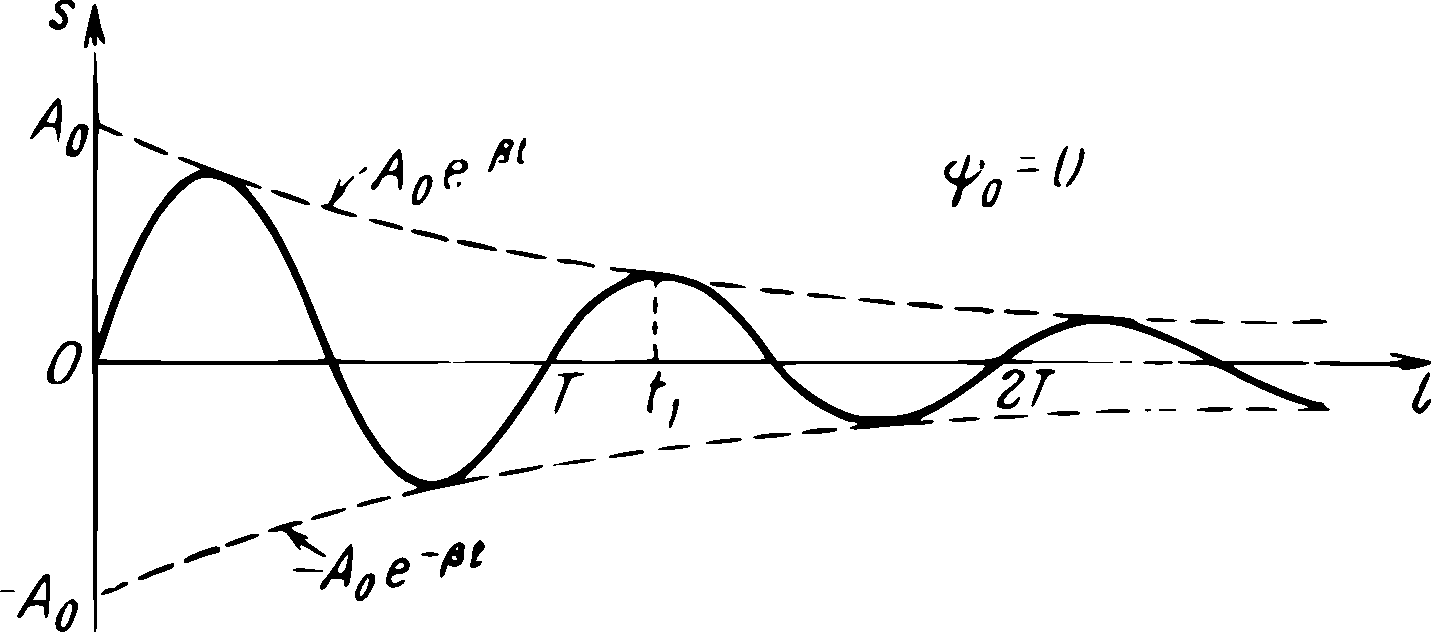
\includegraphics[width=0.9\textwidth]{figs/ch-29/fig-29-01.pdf}
\sidecaption{The curve of the dependence of s on $t$ at $\psi_{0} = 0$ for damped oscillations.\zhcap{阻尼振动中 $s$ 随 $t$ 变化的曲线（$\psi_{0} = 0$）。}\label{fig-29-01}}
\end{figure}


Damped oscillations are not periodical ones \ssect{28.1.2}. For example, the maximum value of the varying quantity $s$, reached at a certain instant $t_{1}$ of time, is never repeated subsequently
(at $t > t_{1}$). But the quantity $s$ becomes zero in damped oscillation as it varies in a single direction (decreases, for instance) and also reaches its maximum and minimum values after \redem{equal} time intervals. Thus
\zhpar{阻尼振动不是周期性振动（\ssect{28.1.2}）。例如，变化量 $s$ 在某一时刻 $t_{1}$ 达到的最大值，此后（$t > t_{1}$）再也不会重复出现。但在阻尼振动中，量 $s$ 在沿单一方向变化（例如减小）的同时会变为零，并且以\redem{相等}的时间间隔达到其极大值和极小值。于是}
\begin{equation*}%
T = \frac{2\pi}{\omega} = \frac{2 \pi}{\sqrt{\omega_{0}^{2} - \beta^{2}}}.
\end{equation*}
For this reason, the quantities $T$ and $\omega$ are conditionally called the \redem{period (conditional period)} and \redem{angular frequency (conditional angular frequency) of damped oscillation}.
\zhpar{因此，$T$ 和 $\omega$ 被称为阻尼振动的\redem{周期（条件周期）}和\redem{角频率（条件角频率）}。}

The quantity
\zhpar{下式所示的量}
\begin{equation*}%
A = A_{0} \exp(-\beta t)
\end{equation*}
Is called the \redem{amplitude of damped oscillation}, where $A_{0}$ is the initial amplitude. The amplitude of damped oscillation decreases in the course of time; the greater the damping factor $\beta$, the more rapidly the amplitude decreases.
\zhpar{被称为\redem{阻尼振动的振幅}，式中 $A_{0}$ 为初始振幅。阻尼振动的振幅随时间减小；阻尼因子 $\beta$ 越大，振幅减小得越快。}

The time interval $\tau = 1/\beta$ during which there is an $e$-fold decrease in the amplitude of damped oscillation, is called the \redem{relaxation time}.
\zhpar{振幅减小 $e$ 倍（即减小为原来的 $1/e$）所经历的时间间隔 $\tau = 1/\beta$ 称为\redem{弛豫时间}。}

\subsection{}\label{29.1.4} \redem{The logarithmic decrement of damping} is the dimensionless quantity $\delta$, equal to the natural logarithm of the ratio of the amplitudes of damped oscillation at the instants of time $t$ and $t + T$ (where $T$ is the conditional period of oscillation). Thus
\zhpar{\redem{阻尼的对数减缩}是一个无量纲量 $\delta$，它等于时刻 $t$ 与 $t + T$（其中 $T$ 为条件振动周期）时阻尼振动振幅之比的自然对数。即}
\begin{equation*}%
\delta =\ln \frac{A(t)}{A(t+ T)} = \beta T = \frac{T}{\tau} = \frac{1}{N},
\end{equation*}
where $N$ is the number of oscillations in which the amplitude is reduced $e$-fold.
\zhpar{式中 $N$ 为振幅减小 $e$ 倍时所经历的振动次数。}

The relation between the angular frequency $\omega$ of damped oscillation of a system and the logarithmic decrement of damping $\delta$ is
\zhpar{阻尼振动系统的角频率 $\omega$ 与阻尼的对数减缩 $\delta$ 之间的关系为：}
\begin{equation*}%
\omega = \omega_{0} \sqrt{1 - \left( \frac{\omega}{\omega_{0}}\right)^{2} \,  \left( \frac{\delta}{2\pi}\right)^{2}}.
\end{equation*}


\subsection{}\label{29.1.5} \redem{The $Q$ factor (or quality factor or storage factor)} of an oscillatory system is the dimensionless quantity $Q$, equal to the product of $2\pi$ by the ratio of the energy of oscillation $E (t)$ of the system at the arbitrary time instant $t$ to the decrease of this energy during the length of time from $t$ to $t + T$, i.e. during one conditional period of damped oscillation. Thus
\zhpar{振动系统的\redem{$Q$ 因子}（或称品质因数、储能因子）是一个无量纲量 $Q$，它等于 $2\pi$ 与以下两者之比的乘积：系统在任意时刻 $t$ 的振动能量 $E (t)$，与从 $t$ 到 $t + T$ 这段时间（即阻尼振动的一个条件周期）内该能量的减少量之比。即}
\begin{equation*}%
Q = 2 \pi \frac{E(t)}{E(t) - E(t+T)}.
\end{equation*}
Since the energy $E (t)$ is proportional to the square of the amplitude $A (t)$ of the oscillation,
\zhpar{由于能量 $E (t)$ 与振动振幅 $A (t)$ 的平方成正比，}
\begin{align*}%
Q & = 2 \pi \frac{A^{2}(t)}{A^{2}(t) - A^{2}(t+T)} = \frac{2\pi}{1 - \exp(-2 \beta T)}\\ 
& = \frac{2\pi}{1 - \exp(-2\delta)}.
\end{align*}
At low values of the logarithmic decrement of damping $\delta$, the $Q$ factor of an oscillatory system is $Q = \pi/\delta$. Here the conditional period of damped oscillation $T$ is practically equal to the period $T_{0}$ of free undamped oscillation and, consequently, $Q = \pi/\beta T_{0} = \omega_{0}/2\beta$. For example, the $Q$ factor of an electrical
oscillatory circuit \ssect{28.3.1} is $Q = \sqrt{L/C}/R$, and that of a spring pendulum \ssect{29.1.2} is $Q = \sqrt{km}/b$.
\zhpar{当阻尼的对数减缩 $\delta$ 较小时，振动系统的 $Q$ 因子为 $Q = \pi/\delta$。此时阻尼振动的条件周期 $T$ 实际上等于无阻尼自由振动的周期 $T_{0}$，因而 $Q = \pi/\beta T_{0} = \omega_{0}/2\beta$。例如，电振荡回路（\ssect{28.3.1}）的 $Q$ 因子为 $Q = \sqrt{L/C}/R$，弹簧振子（\ssect{29.1.2}）的 $Q$ 因子为 $Q = \sqrt{km}/b$。}

\subsection{}\label{29.1.6} The conditional period of damped oscillation increases with the damping factor $\beta$ and becomes infinite at $\beta = \omega_{0}$. If $\beta > \omega_{0}$ the differential equation of motion of the system
\zhpar{阻尼振动的条件周期随阻尼因子 $\beta$ 的增大而增大，并在 $\beta = \omega_{0}$ 时变为无穷大。若 $\beta > \omega_{0}$，则系统的运动微分方程}
\begin{equation*}%
\dv[2]{s}{t} + 2\beta \dv{s}{t} + \omega_{0}^{2} s = 0,
\end{equation*}
has the following general solution: 
\zhpar{其通解具有如下形式：}
\begin{equation*}%
s = C_{1} \exp(-\alpha_{1}t) + C_{2} \exp(-\alpha_{2}t),
\end{equation*}
where $\alpha_{1} = \beta + \sqrt{\beta^{2} - \omega_{0}^{2}}$,  $\alpha_{2} = \beta - \sqrt{\beta^{2} - \omega_{0}^{2}}$ and $C_{1}$ and $C_{2}$ are constant factors depending upon the initial conditions. If the initial values (at the instant of time $t = 0$) equal: $s = s_{0}$ and $\dv*{s}{t} = v_{0}$, then
\zhpar{式中 $\alpha_{1} = \beta + \sqrt{\beta^{2} - \omega_{0}^{2}}$，$\alpha_{2} = \beta - \sqrt{\beta^{2} - \omega_{0}^{2}}$，$C_{1}$ 和 $C_{2}$ 为取决于初始条件的常量因子。若初始时刻（$t = 0$）的取值为 $s = s_{0}$ 和 $\dv*{s}{t} = v_{0}$，则}
\begin{equation*}%
C_{1} = -\frac{\alpha_{2}s_{0} + v_{0}}{\alpha_{1} - \alpha_{2}} \qand C_{2} = \frac{\alpha_{1}s_{0} + v_{0}}{\alpha_{1} - \alpha_{2}} 
\end{equation*}
Such motion of the system is not of an oscillatory nature and is said to be \redem{aperiodic}. Depending upon the initial conditions, aperiodic motion of the system may be either of two kinds (\figr{fig-29-02}). Type $a$ motion occurs when $s_{0}$ and $v_{0}$ are opposite in sign and $\abs{v_{0}} > \alpha_{1} \abs{s_{0}}$. Otherwise, the aperiodic motion is of the $b$ type.
\zhpar{这种运动不具有振动（振荡）的性质，称为\redem{非周期}运动。根据初始条件的不同，系统的非周期运动可分为两种类型（见\figr{fig-29-02}）。当 $s_{0}$ 与 $v_{0}$ 符号相反且 $\abs{v_{0}} > \alpha_{1} \abs{s_{0}}$ 时，为 $a$ 型运动；否则为 $b$ 型运动。}

\begin{marginfigure}[-2cm]
\centering
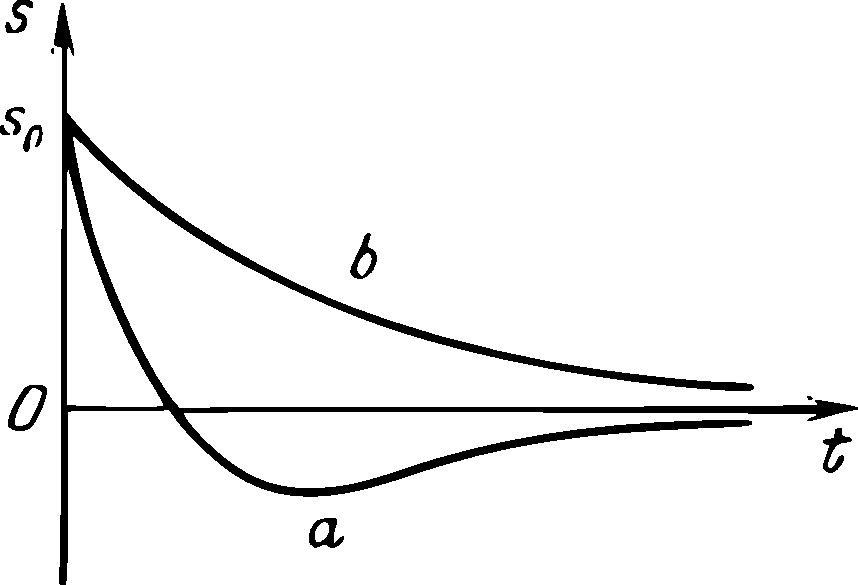
\includegraphics[width=0.8\textwidth]{figs/ch-29/fig-29-02.pdf}
\sidecaption{The different types of aperiodic motions.\zhcap{不同类型的非周期运动。}\label{fig-29-02}}
\end{marginfigure}

\section{Forced Mechanical Vibration}
\label{sec-29.2} 
\zhtitle{受迫机械振动}



\subsection{}\label{29.2.1} A variable external force, applied to a system and causing its forced mechanical vibration, is called the \redem{disturbing}, or \redem{driving}, force.
\zhpar{随时间变化的外力作用于系统并引起其受迫机械振动，称为\redem{扰动力}，或\redem{驱动力}。}

The \redem{differential equation of forced vibration} (or \redem{oscillation}) of the simplest linear system \ssect{29.1.1}, the spring pendulum \ssect{29.1.2}, executed along the $OX$ axis due to the action of the variable external force $\vb{F} (t)$ is:
\zhpar{最简单的线性系统（\ssect{29.1.1}），即沿 $OX$ 轴运动的弹簧振子（\ssect{29.1.2}），在变化外力 $\vb{F} (t)$ 作用下做受迫振动（或振荡），其\redem{受迫振动微分方程}为：}
\begin{equation*}%
\dv[2]{x}{t} + 2\beta \dv{x}{t} + \omega_{0}^{2} x = \frac{1}{m} \, F_{x}(t).
\end{equation*}

If $F_{x} (t)$ is a periodic function of time, then, after application of the force to the pendulum, the \redem{forced vibration} begins \redem{with a transient condition}. The pendulum simultaneously participates in two vibrations:
\zhpar{若 $F_{x} (t)$ 为时间的周期函数，则在对摆施加外力后，受迫振动\redem{以过渡过程开始}。摆同时参与两种振动：}
\begin{equation*}%
x = x_{1}(t) + x_{2}(t)
\end{equation*}
The first term corresponds to free damped oscillation\sidenote{It is assumed that $\beta < \omega_{0}$. Otherwise, the free motion of the pendulum would be aperiodic \ssect{29.1.6}, i.e.
\begin{align*}
x_{1}(t) &= C_{1} \exp \left(-(\beta + \sqrt{\beta^{2} - \omega_{0}^{2}}) t\right) \\
&\quad + C_{2} \exp \left(-(\beta - \sqrt{\beta^{2} - \omega_{0}^{2}}) t\right).
\end{align*}
} of the pendulum \ssect{29.1.3}:
\zhpar{第一项对应于摆的自由阻尼振动（\ssect{29.1.3}）：}
\zhpar{注：假定 $\beta < \omega_{0}$。否则摆的自由运动将是非周期的（见\ssect{29.1.6}），其解为两个指数项之和。}
\begin{equation*}%
x_{1}(t) = A_{0} \exp(- \beta t) \sin (\omega t + \psi_{0}),
\end{equation*}
where $\omega = \sqrt{\omega_{0}^{2} - \beta^{2}}$.
\zhpar{式中 $\omega = \sqrt{\omega_{0}^{2} - \beta^{2}}$。}

The second term corresponds to the undamped periodic oscillation of the pendulum at a frequency equal to that of the driving force $F_{x} (t)$.
\zhpar{第二项对应于摆以与驱动力 $F_{x} (t)$ 相同的频率做的无阻尼周期振动。}

The amplitude value of $x_{1} (t)$, equal to $A_{0} \exp (-\beta t)$, is reduced at a more or less rapid rate after the beginning of the forced vibration (or oscillation). During the time $\tau = 4.6/\beta$ the amplitude of $x_{1} (t)$ decreases by a factor of 100. Consequently, after a certain time $\tau$ following the beginning of vibration $(\tau \approx \tau_{0})$, free vibration of the pendulum practically ceases: $x (t) \approx x_{2}(t)$. The pendulum reaches a state of \redem{steady forced vibration} (or oscillation) at the frequency of the driving force.
\zhpar{$x_{1} (t)$ 的振幅 $A_{0} \exp (-\beta t)$ 从受迫振动开始后便以或快或慢的速率减小。在 $\tau = 4.6/\beta$ 的时间内，$x_{1} (t)$ 的振幅减小为原来的 $1/100$。因此，受迫振动开始后经过一段时间 $\tau$（$\tau \approx \tau_{0}$）之后，摆的自由振动实际上停止：$x (t) \approx x_{2}(t)$。摆达到以驱动力频率进行的\redem{稳态受迫振动}（或振荡）状态。}

\subsection{}\label{29.2.2} When the driving force varies according to a harmonic law, i.e. $F_{x} = F_{0}\cos \Omega t$, the steady-state forced vibration of the pendulum is also harmonic at the same frequency. Thus
\zhpar{当驱动力按简谐规律变化，即 $F_{x} = F_{0}\cos \Omega t$ 时，摆的稳态受迫振动同样为简谐振动，且频率相同。于是}
\begin{equation*}%
x = A \cos (\Omega t + \varphi_{0}).
\end{equation*}
The amplitude $A$ of this vibration and the phase shift $\varphi_{0}$ between the displacement and the driving force depend upon the relation between the angular frequencies of the forced vibration $(\Omega)$ and the free undamped vibration $(\omega_{0})$ of the pendulum. Thus
\zhpar{该振动的振幅 $A$ 以及位移与驱动力之间的相位差 $\varphi_{0}$，取决于受迫振动角频率 $(\Omega)$ 与摆的自由无阻尼振动角频率 $(\omega_{0})$ 之间的关系。二者分别由下列公式给出：}
\begin{align*}%
A &= \frac{F_{0}}{m \sqrt{(\omega_{0}^{2} - \Omega^{2})^{2}+ 4\beta^{2}\Omega^{2}}}, \qand \\ 
\tan \varphi_{0} & = - \frac{2 \beta \Omega}{\omega_{0}^{2} - \Omega^{2}}.
\end{align*}
\begin{marginfigure}[-3cm]
\centering
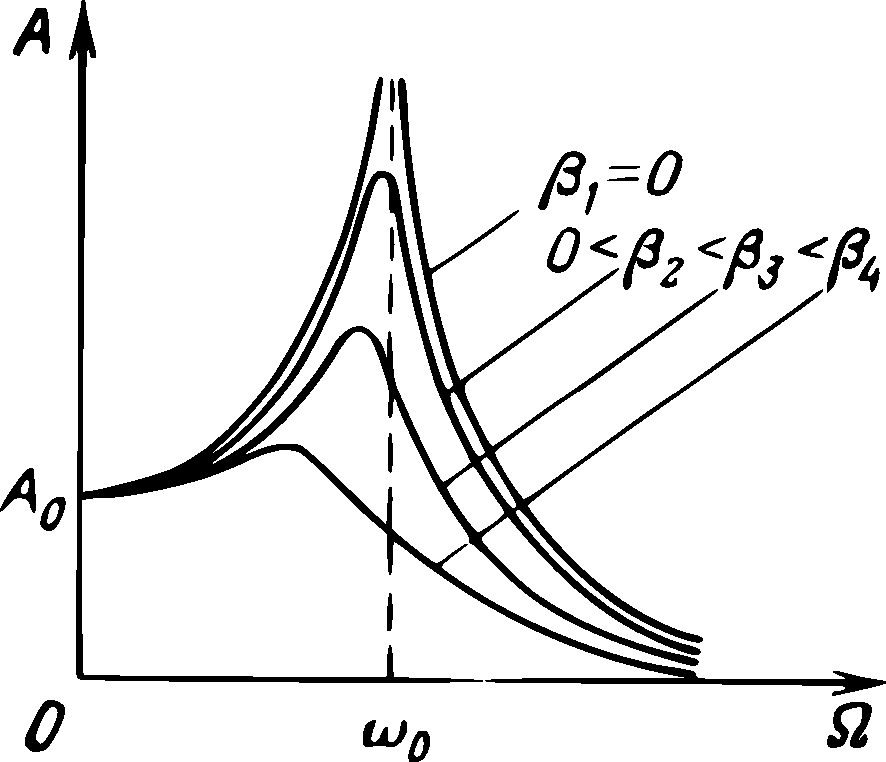
\includegraphics[width=0.8\textwidth]{figs/ch-29/fig-29-03.pdf}
\sidecaption{The curves of the functions $A (\Omega)$ for various values of the damping factor $\beta$.\zhcap{阻尼因子 $\beta$ 取不同值时函数 $A (\Omega)$ 的曲线。}\label{fig-29-03}}
\end{marginfigure}
At $\Omega = 0$ we obtain $\varphi_{0}(0) = 0$ and $A (0) = A_{0}= F_{0}/m\omega_{0}^{2} = F_{0}/k$ which is the \redem{static displacement} of the pendulum from its equilibrium position by the constant force $F_{x} = F_{0}$. At $\Omega \to \infty$, the amplitude $A (\Omega) \to 0$ and $\tan \varphi_{0} \to 0$, whereas $\varphi_{0} \to -\pi$. The curves of the functions $A (\Omega)$ and $\varphi_{0} (\Omega)$ are shown in \figr{fig-29-03} and \figr{fig-29-04} for various values of the damping factor $\beta$.
\zhpar{当 $\Omega = 0$ 时，$\varphi_{0}(0) = 0$，$A (0) = A_{0}= F_{0}/m\omega_{0}^{2} = F_{0}/k$，这就是常力 $F_{x} = F_{0}$ 使摆偏离其平衡位置的\redem{静位移}。当 $\Omega \to \infty$ 时，振幅 $A (\Omega) \to 0$，$\tan \varphi_{0} \to 0$，而 $\varphi_{0} \to -\pi$。函数 $A (\Omega)$ 和 $\varphi_{0} (\Omega)$ 的曲线分别如\figr{fig-29-03}和\figr{fig-29-04}所示，对应于阻尼因子 $\beta$ 的不同取值。}
\begin{marginfigure}[1cm]
\centering
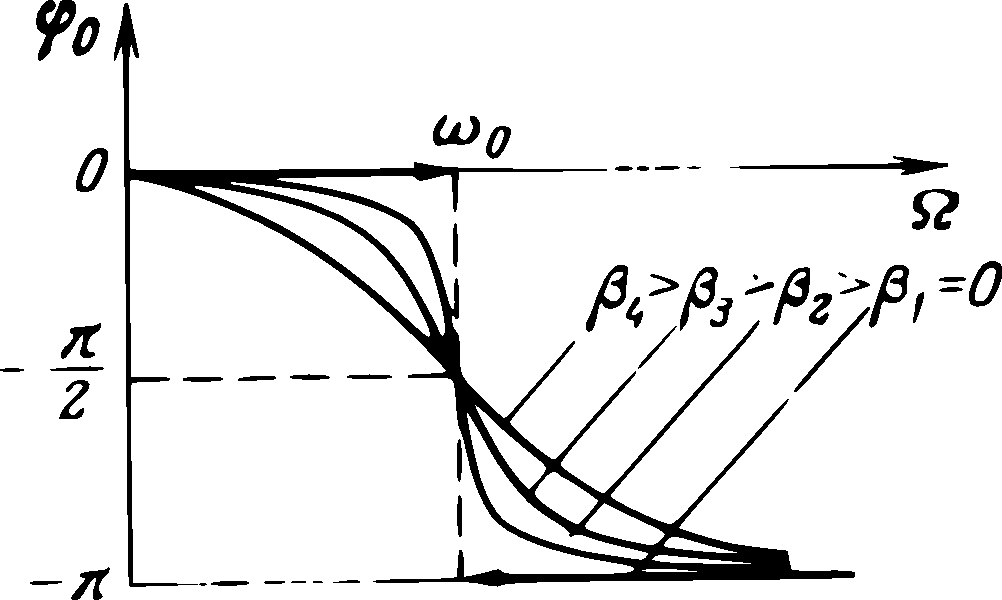
\includegraphics[width=0.9\textwidth]{figs/ch-29/fig-29-04.pdf}
\sidecaption{The curves of the functions $\varphi_{0} (\Omega)$ for various values of the damping factor $\beta$.\zhcap{阻尼因子 $\beta$ 取不同值时函数 $\varphi_{0} (\Omega)$ 的曲线。}\label{fig-29-04}}
\end{marginfigure}

\subsection{}\label{29.2.3} The amplitude of the displacement in the case of steady-state forced harmonic vibration (oscillation) of the pendulum reaches its maximum value at the angular frequency
\zhpar{摆做稳态受迫简谐振动（振荡）时，位移振幅在下式所示的角频率下达到最大值：}
\begin{equation*}%
\Omega_{r} = \sqrt{\omega_{0}^{2} - 2 \beta^{2}} = \sqrt{\omega^{2} - \beta^{2}},
\end{equation*}
where $\omega$ is the angular frequency of free damped vibration of the pendulum \ssect{29.1.3}. The frequency $\Omega_{r}$ is called the \redem{resonance frequency}.
\zhpar{式中 $\omega$ 为摆的自由阻尼振动角频率（\ssect{29.1.3}）。频率 $\Omega_{r}$ 称为\redem{共振频率}。}

The maximum amplitude is
\zhpar{最大振幅为}
\begin{equation*}%{
A_{\text{max}} = A(\Omega_{r}) = \frac{F_{0}}{2m\beta \omega} = \frac{\pi F_{0}}{m\delta \omega^{2}},
\end{equation*}
where $\delta$ is the logarithmic decrement of damping \ssect{29.1.4}. When $\beta \ll \omega_{0}$, $\Omega_{r} \approx \omega_{0}$
$\varphi_{0}(\Omega_{r}) \approx  -\pi/2$, and $A_{\text{max}} \approx Q A_{0}$, where $Q  \approx \pi/\delta$ is the $Q$ factor of the pendulum \ssect{29.1.5} and $A_{0}$ is the static displacement \ssect{29.2.2}.
\zhpar{式中 $\delta$ 为阻尼的对数减缩（\ssect{29.1.4}）。当 $\beta \ll \omega_{0}$ 时，$\Omega_{r} \approx \omega_{0}$，$\varphi_{0}(\Omega_{r}) \approx  -\pi/2$，且 $A_{\text{max}} \approx Q A_{0}$，其中 $Q  \approx \pi/\delta$ 为摆的 $Q$ 因子（\ssect{29.1.5}），$A_{0}$ 为静位移（\ssect{29.2.2}）。}

The drastic increase in the amplitude of forced mechanical vibration (or oscillation) as the angular frequency of the driving force approaches the value $\Omega_{r}$ is the phenomenon called \redem{mechanical resonance}. Accordingly, the curves of the dependence of $A$ on $\Omega$, shown in \figr{fig-29-03} are called \redem{resonance curves}.
\zhpar{当驱动力的角频率趋近于 $\Omega_{r}$ 时，受迫机械振动（或振荡）的振幅急剧增大，这种现象称为\redem{机械共振}。相应地，如\figr{fig-29-03}所示的 $A$ 随 $\Omega$ 变化的曲线称为\redem{共振曲线}。}

As the damping factor $\beta$ is increased, the peaks on the resonance curves are rapidly reduced (at small $\beta$ values the amplitude $A_{\text{max}} \approx 1/\beta$) and the resonance frequency $\Omega_{r}$ is slowly decreased.
\zhpar{随着阻尼因子 $\beta$ 的增大，共振曲线上的峰值迅速降低（当 $\beta$ 较小时，振幅 $A_{\text{max}} \approx 1/\beta$），而共振频率 $\Omega_{r}$ 缓慢减小。}

\subsection{}\label{29.2.4} The \redem{velocity of the pendulum} in steady-state forced harmonic vibration (oscillation) is
\zhpar{摆在稳态受迫简谐振动（振荡）中的\redem{速度}为：}
\begin{equation*}%
v_{x} = \dv{x}{t} = - A \Omega \sin ( \Omega t + \varphi_{0}) = A_{v}\cos(\Omega t + \alpha).
\end{equation*}
Here $A_{v} = A\Omega$ and $\alpha = \varphi_{0} + \pi/2$ are the amplitude of the velocity and the phase difference between the velocity and the driving force:
\zhpar{式中 $A_{v} = A\Omega$ 和 $\alpha = \varphi_{0} + \pi/2$ 分别为速度振幅以及速度与驱动力之间的相位差：}
\begin{align*}%
A_{v} &= \frac{F_{0}\Omega}{m \sqrt{(\omega_{0}^{2} - \Omega^{2})^{2}+ 4\beta^{2}\Omega^{2}}}\\ &=  \frac{F_{0}}{m \sqrt{\dfrac{(\omega_{0}^{2} - \Omega^{2})^{2}}{\Omega^{2}} + 4 \beta^{2}}}, \qand \\ 
\tan \alpha & = -\cot \varphi_{0} = \frac{\omega_{0}^{2} - \Omega^{2}}{2 \beta \Omega}.
\end{align*}
The amplitude of the velocity is maximal at $\Omega = \omega_{0}$ and equals
\zhpar{速度振幅在 $\Omega = \omega_{0}$ 时最大，其值为}
\begin{equation*}%
(A_{v})_{\text{max}} = A_{v} (\omega_{0}) = \frac{F_{0}}{2m \beta}.
\end{equation*}
In this case, $\alpha = 0$, i.e. the velocity of the pendulum oscillates in phase with the driving force. As $\Omega \to \infty$, the amplitude $A_{v} \to 0$ and $\alpha \to -\pi/2$, whereas as $\Omega \to 0$, the amplitude $A_{v} \to 0$ and $\alpha \to \pi/2$.
\zhpar{此时 $\alpha = 0$，即摆的速度与驱动力同相振动。当 $\Omega \to \infty$ 时，速度振幅 $A_{v} \to 0$，$\alpha \to -\pi/2$；而当 $\Omega \to 0$ 时，$A_{v} \to 0$，$\alpha \to \pi/2$。}

\subsection{}\label{29.2.5} The \redem{acceleration of the pendulum} in steady-state forced harmonic vibration (oscillation) is
\zhpar{摆在稳态受迫简谐振动（振荡）中的\redem{加速度}为：}
\begin{align*}%
a_{x} & = dv[2]{x}{t} = -A\Omega^{2} \cos (\Omega t + \varphi_{0}) \\
& = A_{a} \cos (\Omega t + \gamma).
\end{align*}
Here $A_{a} = A\Omega^{2}$ and $\gamma = \varphi_{0} + \pi$ are the amplitude of the acceleration and the phase difference between the acceleration and the driving force:
\zhpar{式中 $A_{a} = A\Omega^{2}$ 和 $\gamma = \varphi_{0} + \pi$ 分别为加速度振幅以及加速度与驱动力之间的相位差：}
\begin{equation*}%
A_{a} = \frac{F_{0}\Omega^{2}}{m \sqrt{(\omega_{0}^{2} - \Omega^{2})^{2} + 4 \beta^{2}\Omega^{2}}} = \frac{F_{0}}{m \sqrt{[(\omega_{0}/\Omega)^{2})^{2} - 1]^{2} + (2\beta/\Omega)^{2}}}.
\end{equation*}
The amplitude of acceleration is maximal at 
\zhpar{加速度振幅在下式所示的 $\Omega$ 值处达到最大：}
\begin{equation*}%
\Omega = \frac{\omega_{0}}{\sqrt{1 + (\beta/\omega_{0})^{2}}}  \approx \sqrt{\omega_{0}^{2} - \beta^{2}}.
\end{equation*}
At $\Omega = 0$, the amplitude $A_{a} = 0$, whereas as $\Omega \to \infty$ the amplitude of the acceleration tends to the value $A_{a} (\infty) = F_{0}/m$.
\zhpar{当 $\Omega = 0$ 时，加速度振幅 $A_{a} = 0$；而当 $\Omega \to \infty$ 时，加速度振幅趋于 $A_{a} (\infty) = F_{0}/m$。}

\subsection{}\label{29.2.6} In steady-state forced vibration, the energy loss of the vibratory system, due to dissipative forces \ssect{3.1.7}, is completely compensated by the work performed on the system by the driving force. The work, for example, done in one complete oscillation by the force of resistance acting on the spring pendulum is
\zhpar{在稳态受迫振动中，振动系统因耗散力（\ssect{3.1.7}）而损失的能量，完全由驱动力对系统所做的功来补偿。例如，阻力在弹簧振子的一个完整振动周期内所做的功为}
\begin{align*}%
W_{1} & = -b \int_{0}^{T} \left( \dv{x}{t} \right)^{2} \, \dd t = - 2m \beta A^{2}\Omega^{2} \int_{0}^{T} \sin^{2} (\Omega t + \varphi_{0}) \, \dd t \\
& = -m\beta A^{2} \Omega^{2},
\end{align*}
where $b = 2 m \beta$ is the resistance coefficient \ssect{29.1.2}.
\zhpar{式中 $b = 2 m \beta$ 为阻力系数（\ssect{29.1.2}）。}

The work done during the same time by the driving force $F_{x} = F_{0}\cos \Omega t$ is
\zhpar{同一时间内驱动力 $F_{x} = F_{0}\cos \Omega t$ 所做的功为}
\begin{align*}%
W_{2} & = F_{0} \int_{0}^{T} \dv{x}{t} \cos \Omega t \, \dd t = - A\Omega F_{0} \int_{0}^{T} \cos \Omega t \sin(\Omega t  \varphi_{0}) \, \dd t \\
& = -\frac{1}{2} A \Omega F_{0} \sin \varphi_{0} = - W_{1},
\end{align*}
since $\sin \varphi_{0} = -2m\beta A \Omega/F_{0}$.
\zhpar{由于 $\sin \varphi_{0} = -2m\beta A \Omega/F_{0}$。}

\subsection{}\label{29.2.7} If the driving force acting on the spring pendulum varies periodically, but not according to a harmonic law, it can he represented as the sum of the harmonics of this force \ssect{28.4.6}. These have different amplitudes, initial phases and angular frequencies that are multiples of $\Omega = 2\pi/T$, where $T$ is the period of variation of the driving force. Since the pendulum is a linear vibratory (or oscillatory) system \ssect{29.1.1}, each harmonic of the driving force acts on the system as if there were no other harmonics. Therefore, the steady-state forced oscillation of the pendulum, caused by an arbitrary periodic driving force, can be dealt with as the result of superposing steady-state forced oscillations due to each harmonic component of the driving force acting separately. 
\zhpar{若作用于弹簧振子的驱动力周期性变化但不按简谐规律变化，则可将其表示为该力各次谐波之和（\ssect{28.4.6}）。这些谐波具有不同的振幅和初相位，其角频率为 $\Omega = 2\pi/T$ 的整数倍，其中 $T$ 为驱动力的变化周期。由于摆是线性振动（振荡）系统（\ssect{29.1.1}），驱动力的每个谐波都如同其他谐波不存在时一样作用于系统。因此，摆在任意周期性驱动力作用下的稳态受迫振动，可视为各谐波分量单独作用时所引起的稳态受迫振动的叠加。}

The ``contribution'' of the various harmonic components to the resultant oscillation depends upon their frequency and amplitude. Owing to resonance phenomena, an essential role, is played by only the harmonic components of the driving force that have an angular frequency close to the resonance frequency of the pendulum \ssect{29.2.3}. If the damping factor $\beta$ of the pendulum is small, the pendulum can execute steady-state forced oscillation close to the harmonic one, even if the driving force is far from harmonic. An example of such forced oscillation is that of a pendulum subject to short periodical external action in the form of impacts in a single direction and repeated over equal lengths of time, which are equal to the period of free oscillation of the pendulum.
\zhpar{驱动力各谐波分量对合成振动的“贡献”取决于它们的频率和振幅。由于共振现象，只有角频率接近摆的共振频率（\ssect{29.2.3}）的谐波分量起主要作用。若摆的阻尼因子 $\beta$ 较小，即使驱动力远非简谐，摆也能做接近简谐的稳态受迫振动。此类受迫振动的一个例子是：摆受到沿单一方向的短促周期性冲击，冲击的时间间隔相等，且等于摆的自由振动周期。}

\section{Forced Electrical Oscillation}
\label{sec-29.3}
\zhtitle{受迫电振荡}

\subsection{}\label{29.3.1} To obtain forced oscillation in an electrical oscillatory circuit \ssect{28.3.1} it is necessary to connect into it a source of electrical energy, whose emf $\emf$ varies with time (\figr{fig-29-05}).
\zhpar{为了在电振荡回路（\ssect{28.3.1}）中产生受迫振荡，需要在回路中接入一个电动势 $\emf$ 随时间变化的电能源（见\figr{fig-29-05}）。}
\begin{marginfigure}[1cm]
\centering
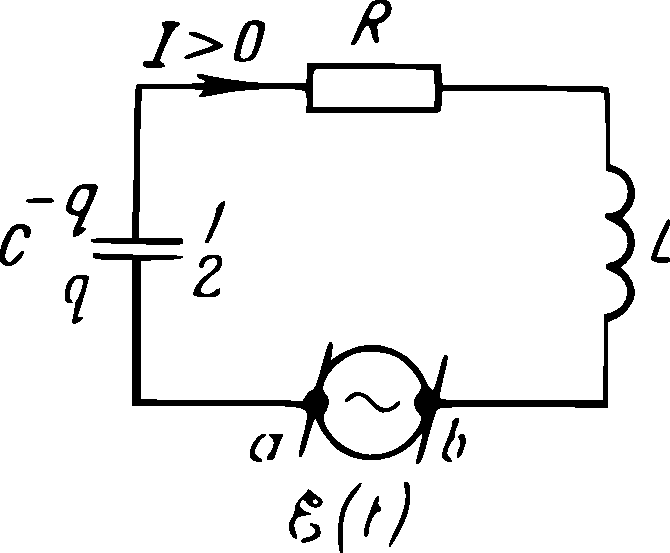
\includegraphics[width=0.9\textwidth]{figs/ch-29/fig-29-05.pdf}
\sidecaption{Setup for obtaining forced electrical oscillaiors with $RLC$ circuit.\zhcap{用 $RLC$ 电路获得受迫电振荡的装置。}\label{fig-29-05}}
\end{marginfigure}

In electrical engineering a source of electrical energy, characterized by its emf and internal electrical resistance, is called a \redem{seat}, or \redem{source, of emf (voltage source)}. According to Ohm's law for the portion $\mathit{1}-R-L-\mathit{2}$ \ssect{21.2.3}, the quasi-stationary current \ssect{28.3.1}, produced in the circuit in forced oscillation, can be found from the formula
\zhpar{在电工技术中，以电动势和内阻为特征的电能源称为\redem{电动势源}，或\redem{电压源}。根据欧姆定律（\ssect{21.2.3}）应用于电路部分 $\mathit{1}-R-L-\mathit{2}$，回路中受迫振荡所产生的准稳电流（\ssect{28.3.1}）可由下式求得：}
\begin{equation}%
IR = V_{1} - V_{2} - L \dv{I}{t} + \emf ( t ) .
\end{equation}
Here $V_{2}- V_{1}= q/C$ is the potential difference across the capacitor plates, $q$ is the capacitor charge, and the internal electrical resistance of the source of emf is assumed to be negligibly small compared to $R$ (such a source of emf is said
to be \redem{ideal}). From the law of conservation of electrical charge \ssect{14.1.3} it follows that $I = \dv*{q}{t}$. Hence, the \redem{differential equation of forced electrical oscillation in a circuit} can be presented in a form similar to the equation for forced mechanical vibration \ssect{29.2.1}:
\zhpar{式中 $V_{2}- V_{1}= q/C$ 为电容器极板间的电势差，$q$ 为电容器的电荷，电动势源的内阻与 $R$ 相比可以忽略不计（这种电动势源称为\redem{理想}电动势源）。由电荷守恒定律（\ssect{14.1.3}）可知 $I = \dv*{q}{t}$。因此，回路中受迫电振荡的\redem{微分方程}可写成与受迫机械振动方程（\ssect{29.2.1}）相似的形式：}
\begin{equation*}%
\dv[2]{q}{t} + 2 \beta \dv{q}{t} + \omega_{0}^{2} q = \frac{1}{L} \emf (t).
\end{equation*}
Here $\beta = R/2L$ is the damping factor for free oscillation in a
circuit, and $\omega_{0} = 1/\sqrt{L C}$ is the angular frequency of free undamped oscillation (i.e. at $R = 0$).
\zhpar{式中 $\beta = R/2L$ 为回路中自由振荡的阻尼因子，$\omega_{0} = 1/\sqrt{L C}$ 为自由无阻尼振荡（即 $R = 0$ 时）的角频率。}

\subsection{}\label{29.3.2} If the driving emf $\emf (t)$ varies according to the harmonic law $\emf (t) = \emf_{0}\cos \Omega t$, then at steady-state forced oscillation \ssect{29.2.1}, the capacitor charge varies harmonically at the same angular frequency $\Omega$:
\zhpar{若驱动电动势 $\emf (t)$ 按简谐规律 $\emf (t) = \emf_{0}\cos \Omega t$ 变化，则在稳态受迫振荡（\ssect{29.2.1}）中，电容器的电荷以相同的角频率 $\Omega$ 作简谐变化：}
\begin{equation*}%
q = q_{0} \cos(\Omega t+ \varphi_{0}).
\end{equation*}
The amplitude $q_{0}$ and the initial phase $\varphi_{0}$ are determined by the formulas
\zhpar{振幅 $q_{0}$ 和初相位 $\varphi_{0}$ 由下列公式确定：}
\begin{align*}%
q_{0} & = \frac{\emf_{0}}{\Omega \sqrt{R^{2} + (\Omega L - 1/\Omega C)^{2}}} = \frac{\emf_{0}}{L \sqrt{(\omega_{0}^{2} - \Omega^{2})^{2} + 4 \beta^{2}\Omega^{2}}} \qand \\
\tan \varphi_{0} & = \frac{R}{\Omega L - 1/\Omega C} = - \frac{2\beta \Omega}{\omega_{0}^{2} - \Omega^{2}}
\end{align*}
At $\Omega = 0$, the phase $\varphi_{0}(0) = 0$ and $q_{0}(0) = \emf_{0}C$ which is the charge of the capacitor at a constant potential difference between the plates equal to $\emf_{0}$. At $\Omega \to \infty$, the amplitude $q_{0}\to 0$, and $\varphi_{0} \to - \pi$. The curves showing the dependence of $\varphi_{0}$ on $\Omega$ are shown in \figr{fig-29-04}, and those of the dependence of $q_{0}$ on $\Omega$, in \figr{fig-29-03}, where $A= q_{0}$ and $A_{0}= q_{0}(0)= \emf_{0}C$.
\zhpar{当 $\Omega = 0$ 时，相位 $\varphi_{0}(0) = 0$，$q_{0}(0) = \emf_{0}C$，即两极板间电势差恒为 $\emf_{0}$ 时电容器的电荷。当 $\Omega \to \infty$ 时，振幅 $q_{0}\to 0$，且 $\varphi_{0} \to - \pi$。$\varphi_{0}$ 随 $\Omega$ 变化的曲线如\figr{fig-29-04}所示，$q_{0}$ 随 $\Omega$ 变化的曲线如\figr{fig-29-03}所示，其中 $A= q_{0}$，$A_{0}= q_{0}(0)= \emf_{0}C$。}

\begin{marginfigure}%[1cm]
\centering
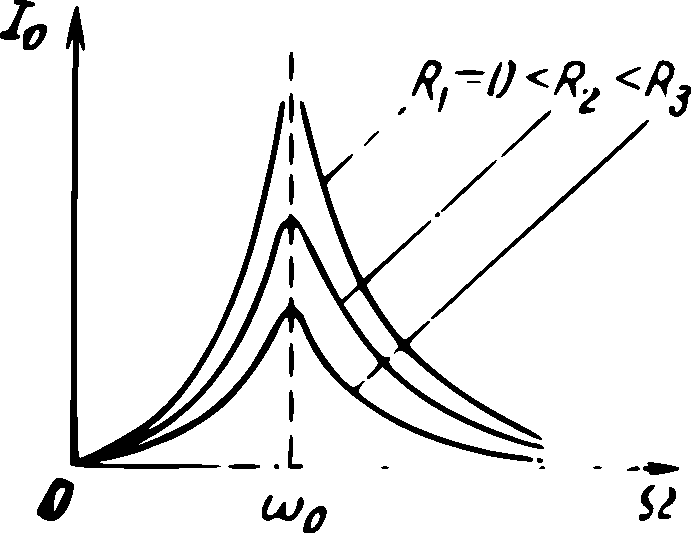
\includegraphics[width=0.9\textwidth]{figs/ch-29/fig-29-06.pdf}
\sidecaption{Resonance curves of the oscillatory circuit.\zhcap{振荡电路的共振曲线。}\label{fig-29-06}}
\end{marginfigure}

\subsection{}\label{29.3.3} With steady-state forced oscillation in the circuit, the current is
\zhpar{电路中做稳态受迫振荡时，电流为}
\begin{equation*}%
I = \dv{q}{t} = - q_{0} \Omega \sin ( \Omega t + \varphi_{0}) = I_{0}\cos (\Omega t - \varphi).
\end{equation*}
The amplitude of the current $I_{0}= q_{0}\Omega$ and the initial phase $-\varphi = \varphi_{0}+ \pi/2$ are determined by the formulas:
\zhpar{电流振幅 $I_{0}= q_{0}\Omega$ 以及初相位 $-\varphi = \varphi_{0}+ \pi/2$ 由下列公式确定：}
\begin{align*}%
I_{0} & = \frac{\emf_{0}}{\sqrt{R^{2} + (\Omega L - 1/\Omega C)^{2}}}\qand \\
\tan \varphi & = \frac{\Omega L - 1/\Omega C}{R}.
\end{align*}
\begin{marginfigure}%[1cm]
\centering
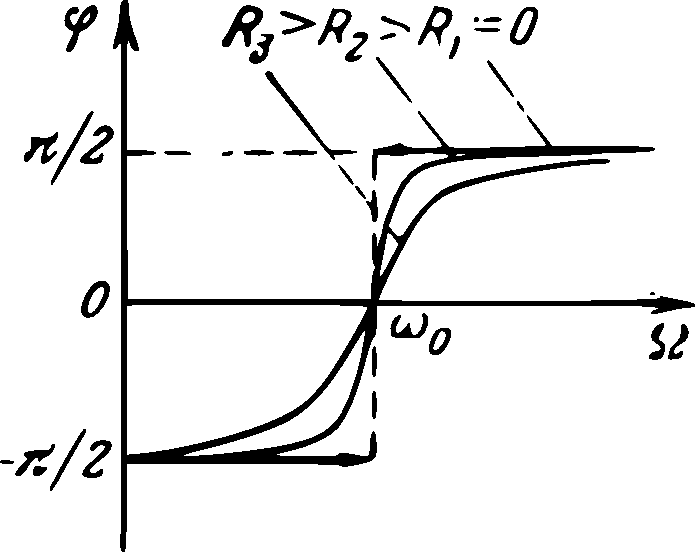
\includegraphics[width=0.9\textwidth]{figs/ch-29/fig-29-07.pdf}
\sidecaption{Curves of the dependence of $\varphi$ on $\Omega$.\zhcap{$\varphi$ 随 $\Omega$ 变化的曲线。}\label{fig-29-07}}
\end{marginfigure}
Curves showing the dependence of $I_{0}$ on $\Omega$ for various values of $R$ are called resonance curves of the oscillatory circuit and are shown in \figr{fig-29-06}; curves of the dependence of $\varphi$ on $\Omega$ are shown in \figr{fig-29-07}. The resonance angular frequency $\Omega_{r}$, corresponding to the maximum amplitude of the current in the circuit in forced oscillation, is independent of $R$. Thus
\zhpar{表示对应于不同 $R$ 值时 $I_{0}$ 随 $\Omega$ 变化关系的曲线称为振荡电路的共振曲线，如\figr{fig-29-06}所示；$\varphi$ 随 $\Omega$ 变化的曲线如\figr{fig-29-07}所示。受迫振荡中对应电路电流振幅最大值的共振角频率 $\Omega_{r}$ 与 $R$ 无关，即}
\begin{equation*}%
\Omega_{r} = \omega_{0} = \frac{1}{\sqrt{LC}}.
\end{equation*}
The current amplitude at resonance is $I_{0}(\Omega_{r}) = \emf_{0}/R$, and the phase difference between the current and emf is $\varphi (\Omega_{r}) = 0$. When $\Omega < \omega_{0}$, $\varphi < 0$, i.e. the current leads the emf in phase; the lower the frequency $\Omega$, the greater this phase lead ($\varphi = -\pi/2$ at  $\Omega = 0$). When $\Omega > \varphi_{0}$, ($ \varphi > 0$, i.e. the current lags in phase behind the emf; the higher the frequency $\Omega$, the greater this phase lag ($\varphi \to \pi/2$ as $\Omega \to \infty$).
\zhpar{共振时电流振幅为 $I_{0}(\Omega_{r}) = \emf_{0}/R$，电流与电动势之间的相位差为 $\varphi (\Omega_{r}) = 0$。当 $\Omega < \omega_{0}$ 时，$\varphi < 0$，即电流在相位上超前于电动势；频率 $\Omega$ 越低，这种相位超前越大（当 $\Omega = 0$ 时 $\varphi = -\pi/2$）。当 $\Omega > \varphi_{0}$ 时（$\varphi > 0$），即电流在相位上滞后于电动势；频率 $\Omega$ 越高，这种相位滞后越大（当 $\Omega \to \infty$ 时 $\varphi \to \pi/2$）。}

\subsection{}\label{29.3.4} The potential difference across the terminals $a$ and $b$ of an ideal source of harmonic emf (\figr{fig-29-05}) is equal to its emf. Thus
\zhpar{理想谐变电动势源（见\figr{fig-29-05}）两端 $a$ 与 $b$ 之间的电势差等于其电动势。于是}
\begin{equation*}%
u = V_{a} - V_{b} = \emf_{0} \cos \Omega t.
\end{equation*}
The potential drops across various portions of the circuit illustrated in \figr{fig-29-05} and having the variable sinusoidal (harmonic) current $I = I_{0}\cos (\Omega t - \varphi)$, a capacitor of capacitance $C$, resistor of resistance $R$ and a coil of inductance $L$ are as follows:
\zhpar{在\figr{fig-29-05}所示电路中，对于通有交变正弦（谐变）电流 $I = I_{0}\cos (\Omega t - \varphi)$ 的各部分（分别为电容为 $C$ 的电容器、电阻为 $R$ 的电阻以及电感为 $L$ 的线圈），其电势降落分别为：}
\begin{align*}%
u_{C} & = V_{2} - V_{1} = \frac{q}{C} = U_{C} \cos \left( \Omega t - \varphi - \frac{\pi}{2} \right), \\ 
u_{R} & = IR =  U_{R} \cos ( \Omega t - \varphi), \\ 
u_{L} & = L \dv{I}{t} = U_{L} \cos \left( \Omega t - \varphi + \frac{\pi}{2} \right).
\end{align*}
The variation of $u_{R}$ is in phase with that of current $I$ in the circuit, $u_{L}$ leads the current in phase by $\pi/2$, and $u_{C}$ lags behind the current in phase by $\pi/2$. Here
\zhpar{$u_{R}$ 的变化与电路中电流 $I$ 同相，$u_{L}$ 在相位上超前电流 $\pi/2$，$u_{C}$ 在相位上滞后电流 $\pi/2$。于是}
\begin{equation*}%
u_{C} + u_{R} + u_{L} = u =  \emf_{0} \cos \Omega t.
\end{equation*}

\subsection{}\label{29.3.5} The amplitude values of $u_{C}$ , $u_{L}$ and $u_{R}$ are equal, respectively, to
\zhpar{$u_{C}$、$u_{L}$ 和 $u_{R}$ 的振幅值分别等于}
\begin{equation*}%
U_{C} = X_{C}I_{0}, \quad U_{L}= X_{L}I_{0} \qand U_{R}  =RI_{0}.
\end{equation*}
where $X_{C} = 1/\Omega C$ is the \redem{capacitive reactance} of the circuit, and $X_{L} = \Omega L$ is the \redem{inductive reactance} of the circuit. The quantity $X = X_{L} - X_{C} = \Omega L - 1/\Omega C$ is called the \redem{reactance of the circuit}, $R$ is called the \redem{resistance} and $Z = \sqrt{ R^{2} + (\Omega L - 1/\Omega C)^{2}}$ is called its \redem{impedance}.
\zhpar{式中 $X_{C} = 1/\Omega C$ 为电路的\redem{容抗}，$X_{L} = \Omega L$ 为电路的\redem{感抗}。量 $X = X_{L} - X_{C} = \Omega L - 1/\Omega C$ 称为电路的\redem{电抗}，$R$ 称为\redem{电阻}，$Z = \sqrt{ R^{2} + (\Omega L - 1/\Omega C)^{2}}$ 称为其\redem{阻抗}。}

The formulas in \ssect{29.3.3} for the amplitude of the sinusoidal current in the circuit and its initial phase can be rewritten in the form: 
\zhpar{\ssect{29.3.3}中给出的正弦电流振幅及其初相位的公式可改写为下列形式：}
\begin{equation*}%
I_{0} = \frac{\emf_{0}}{Z} \qand \tan \varphi = \frac{X}{R},
\end{equation*}
with $\cos \varphi = R/Z$ and $\sin \varphi = X/Z$. 
\zhpar{其中 $\cos \varphi = R/Z$，$\sin \varphi = X/Z$。}

At resonance $\Omega = 1/\sqrt{LC}$ and $X_{L} = X_{C}$,so that the reactance of the circuit becomes zero and the impedance reaches its minimum value, which is equal to the resistance $R$. Thus
\zhpar{共振时 $\Omega = 1/\sqrt{LC}$，且 $X_{L} = X_{C}$，因此电路的电抗为零，阻抗达到其最小值，等于电阻 $R$。于是}
\begin{equation*}%
X (\Omega_{r}) = 0 \qand Z (\Omega_{r}) = Z_{\text{min}} = R.
\end{equation*}
In this case $U_{R} = 0$ and $U_{C} = U_{L} = \sqrt{L/C}\, \emf_{0}/R$.
\zhpar{此时 $U_{R} = 0$，且 $U_{C} = U_{L} = \sqrt{L/C}\, \emf_{0}/R$。}

\subsection{}\label{29.3.6} The \redem{effective value of a periodic current} (and, accordingly, the emf, voltage, etc.) is the root-mean-square value of the current during the time $T$ of its variation. Thus
\zhpar{周期性电流（以及相应的电动势、电压等）的\redem{有效值}是其变化周期 $T$ 内电流的均方根值。即}
\begin{equation*}%
I_{\text{eff}} = \sqrt{\frac{1}{T}\int_{0}^{T} I^{2} \, \dd t }
\end{equation*}
For a sinusoidal current and a sinusoidal emf
\zhpar{对于正弦电流和正弦电动势，}
\begin{equation*}%
I_{\text{eff}} = \frac{I_{0}}{\sqrt{2}} \qand \emf_{\text{eff}}
 = \frac{\emf_{0}}{\sqrt{2}}. 
\end{equation*}
An element of work done by sinusoidal current during the short time $\dd t$ in the circuit illustrated in \figr{fig-29-05} is equal to
\zhpar{在\figr{fig-29-05}所示电路中，正弦电流在短时间 $\dd t$ 内所做功的微元为}
\begin{equation*}%
\delta W = I u \, \dd t = I_{0}\emf_{0} \cos (\Omega t - \varphi) \, \cos \Omega t \, \dd t.
\end{equation*}
The \redem{instantaneous power of the current in the circuit} is
\zhpar{电路中电流的\redem{瞬时功率}为}
\begin{equation*}%
P_{\text{ins}} = \frac{\delta W}{\dd t} - Iu = I_{0}\emf_{0} \cos (\Omega t - \varphi) \, \cos \Omega t.
\end{equation*}
The average value of the instantaneous power during a period is called the \redem{active}, or \redem{true, power} $P$ of the current in the electric circuit. Thus
\zhpar{瞬时功率在一个周期内的平均值称为电路中电流的\redem{有功功率}，或\redem{真功率} $P$。即}
\begin{align*}%
P & = \frac{1}{T} \int_{0}^{T} P_{\text{ins}} \, \dd t = \frac{1}{2} I_{0}\emf_{0} \cos \varphi \\
& = I_{\text{eff}}\emf_{\text{eff}} \cos \varphi.
\end{align*}
The factor $\cos \varphi$ is called the \redem{power factor}. Since $I_{\text{eff}} = \emf_{\text{eff}}/Z$ and $\cos \varphi = R/Z$,
\zhpar{因子 $\cos \varphi$ 称为\redem{功率因数}。由于 $I_{\text{eff}} = \emf_{\text{eff}}/Z$ 且 $\cos \varphi = R/Z$，故}
\begin{equation*}%
P  = \frac{R}{Z^{2}}\emf_{\text{eff}}^{2}.
\end{equation*}
At resonance $Z = R$ and the active power reaches its maximum value
\zhpar{共振时 $Z = R$，有功功率达到其最大值：}
\begin{equation*}%
P  = \frac{\emf_{\text{eff}}^{2}}{R} = \frac{\emf_{0}^{2}}{2R}.
\end{equation*}

